\documentclass[border=10pt]{standalone}
\usepackage{fontspec}
\setmainfont{Carlito}
\usepackage{unicode-math}
\setmathfont{Latin Modern Math}
\usepackage{xcolor}
\usepackage{tikz}
\usetikzlibrary{positioning, arrows.meta, calc}

\definecolor{canvabg}{RGB}{246,244,241}
\definecolor{trough}{RGB}{160,55,50}
\definecolor{bridge}{RGB}{30,90,140}
\definecolor{accent}{RGB}{18,125,108}
\definecolor{textDark}{RGB}{40,40,40}
\definecolor{textMute}{RGB}{125,120,113}

\pagecolor{canvabg}

\begin{document}
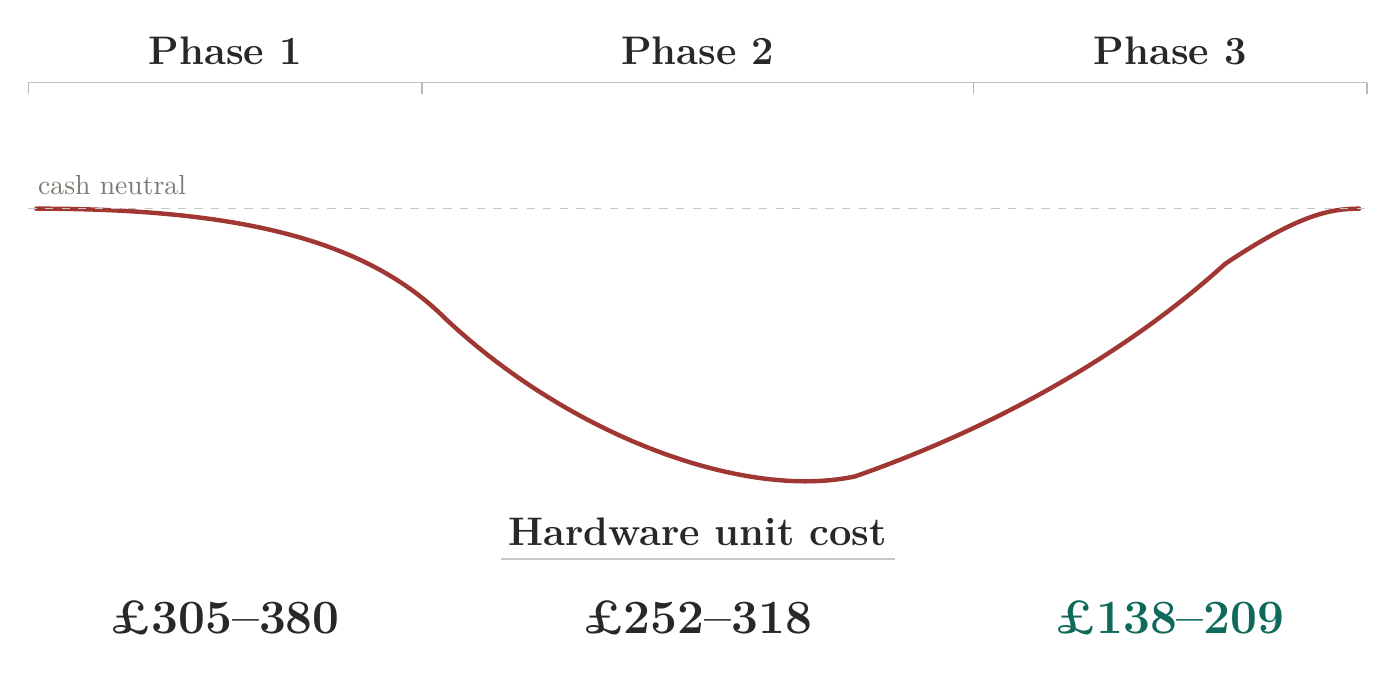
\begin{tikzpicture}[
    every node/.style={text=textDark},
]
% Canvas: x in [0, 18], y in [0, 9]

% --- Phase axis (top): labels + light tick marks ---
\draw[gray!50, line width=0.5pt] (0.5, 8.0) -- (17.5, 8.0);
\foreach \x in {0.5, 5.5, 12.5, 17.5} {
    \draw[gray!55, line width=0.5pt] (\x, 8.0) -- (\x, 7.85);
}

\node[anchor=south, font=\bfseries\Large] at (3.0,  8.10) {Phase 1};
\node[anchor=south, font=\bfseries\Large] at (9.0,  8.10) {Phase 2};
\node[anchor=south, font=\bfseries\Large] at (15.0, 8.10) {Phase 3};

% --- Cash-neutral label (line drawn per-state) ---
\node[anchor=south west, font=\normalsize, text=textMute]
    at (0.5, 6.45) {cash neutral};

% --- Cash valley curve ---
\draw[trough, line width=1.6pt, line cap=round]
    (0.6, 6.4)
    .. controls (3.2, 6.4) and (4.8, 6.0) .. (5.8, 5.0)
    .. controls (7.4, 3.5) and (9.6, 2.7) .. (11.0, 3.0)
    .. controls (13.0, 3.7) and (14.6, 4.7) .. (15.7, 5.7)
    .. controls (16.6, 6.3) and (17.0, 6.4) .. (17.4, 6.4);

% --- Hardware unit cost row, treated as a section ---
% Header + thin underline anchor the row so the label doesn't float.
\node[font=\bfseries\Large, text=textDark] at (9.0, 2.30) {Hardware unit cost};
\draw[gray!45, line width=0.5pt] (6.5, 1.95) -- (11.5, 1.95);

\node[font=\bfseries\LARGE, text=textDark]        at (3.0,  1.20) {\pounds 305--380};
\node[font=\bfseries\LARGE, text=textDark]        at (9.0,  1.20) {\pounds 252--318};
\node[font=\bfseries\LARGE, text=accent!85!black] at (15.0, 1.20) {\pounds 138--209};

% Cash-neutral baseline (state 1 only)
\draw[gray!45, line width=0.45pt, dashed] (0.5, 6.4) -- (17.5, 6.4);

\end{tikzpicture}
\end{document}
